\textbf{程序查询方式又称为程序控制I/O方式。}

在这种方式中,数据在CPU和外部设备之间的传送完全靠计算机程序控制,是在CPU主动控制下进行的。当需要输入/输出时,CPU暂停执行主程序,转去执行设备输入/输出的服务程序(指由I/O指令编写成的程序),根据服务程序中的I/O指令进行数据传送。{程序查询方式的主要缺点}在于每时每刻需要不断查询I/O设备是否准备就绪。{下图为}\textbf{单个设备的查询流程}{。}

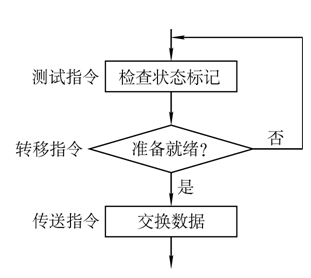
\includegraphics[width=2.39583in,height=2.14583in]{png-jpeg-pics/69E314883DA056493F5A812F4EB1FE08.png}

当I/O设备较多时,CPU需要按各个I/O设备在系统中的优先级别进行逐级查询,其流程如下图所示。下图中设备的优先顺序按1~N降序排列。

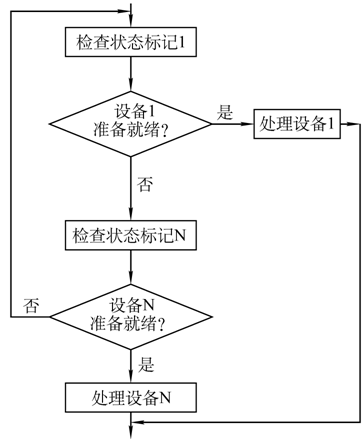
\includegraphics[width=2.39583in,height=2.92708in]{png-jpeg-pics/93AB1CF14106288AE4A3CCD1E3247365.png}

从单个设备的查询流程可以看出,{\textbf{为了正确完成这种查询,通常要执行以下3条指令。}}

\textbf{1)测试指令。}用来查询I/O设备是否准备就绪。

\textbf{2)转移指令。}若I/O设备未准备就绪,则执行转移指令,即转到测试指令,继续测试I/O设备的状态。

\textbf{3)传送指令。}若I/O设备准备就绪,则执行传送指令。\\
